% Formatting of listings
\lstset{language=C, frame=L, basicstyle=\footnotesize,%\sffamily,
	keywordstyle=\bfseries, showstringspaces=false, xleftmargin=\parindent, numbers=none, numberstyle=\tiny, stepnumber=2, numbersep=14pt}
\newpage
\section{Проектирование}
\label{sec:Design}
В ходе проектирования приложения были определены следующие функциональные и нефункциональные требования.
\subsection{Требования к системе}
\label{sec:Requirements}
\textbf{Функциональные требования.}
Функциональные требования описывают, какое поведение должна предоставлять разрабатываемая система.

 \begin{itemizecustom}
 \item Система должна проводить классификацию проектов на основе параметров репозиториев.
 
 \item Пользователи должны иметь возможность просматривать результаты классификации и информацию о проекте.
 
 \item Система должна предоставлять интерфейс для взаимодействия с пользователем.
 \end{itemizecustom}

\textbf{Нефункциональные требования.}

К нефункциональным требованиям системы относятся свойства, которыми она должна обладать. Например, удобство использования, безопасность и т.д.

 \begin{itemizecustom}
 \item Приложение должно иметь интуитивно понятный в использовании пользовательский интерфейс.
 
 \item Основная программная реализация осуществляется с использованием Python.
 
 \item Пользовательский интерфейс должно быть реализовано с использованием веб-сайта.
 \end{itemizecustom}

\subsection{Варианты использования системы}
\label{sec:Using}

Для проектирования приложения был использован язык графического описания для объектного моделирования UML. Была построена модель взаимодействия внешнего актера с приложением в виде диаграммы вариантов использования. В ходе анализа разрабатываемого приложения были выявлены основные варианты использования (рисунок~\ref{ris:variants}).

Для данной диаграммы определен актер -- пользователь, который взаимодействует с приложением. Пользователю доступны следующие варианты использования.

\begin{figure}[h]
    \centering
    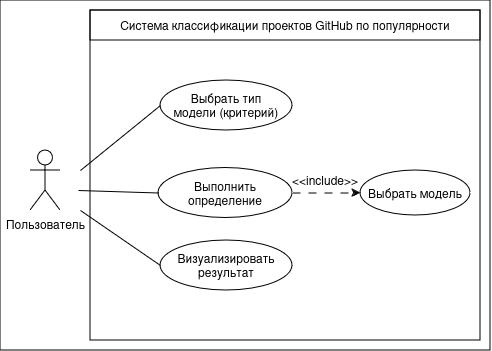
\includegraphics[width=1\linewidth]{pic/variants.png}
    \vspace{-1em}\caption{Варианты использования приложения}
    \label{ris:variants}
\end{figure}
\vspace{1em}
\begin{enumerateparen}
    \item Вариант использования "Выбрать тип модели (критерий)". Пользователь может выбрать тип модели, который будет использоваться для классификации или регрессии. Выбор типа модели определяет метод, который будет применен к входным данным для определения класса популярности или количества звезд.
    
    \item Вариант использования "Выполнить определение". Пользователь может запустить процесс определения класса популярности или количества звезд на основе выбранной модели и входных данных. Данный прецедент включает в себя вариант "Выбрать модель".

    \item Вариант использования "Выбрать модель". Пользователь может выбрать конкретную модель из представленных в системе. Представленные модели могут включать в себя такие методы, как Градиентный бустинг, Случайный лес и другие. 

    \item Вариант использования "Визуализировать результат". Пользователь может визуализировать результаты, представляющие собой класс популярности или количество звезд относительно перечисленных параметров на веб-странице. 
\end{enumerateparen}
Детальная спецификация вариантов использования приложения представлена в приложении А.

\subsection{Архитектура системы}
\label{sec:Architecture}
В данном разделе рассматривается спроектированная архитектура приложения в виде диаграммы компонентов, которая показывает разбиение системы на структурные компоненты.

Спроектированная архитектура приложения представлена на рисунке~\ref{ris:architecture} в виде диаграммы компонентов.

\begin{figure}[h]
    \centering
    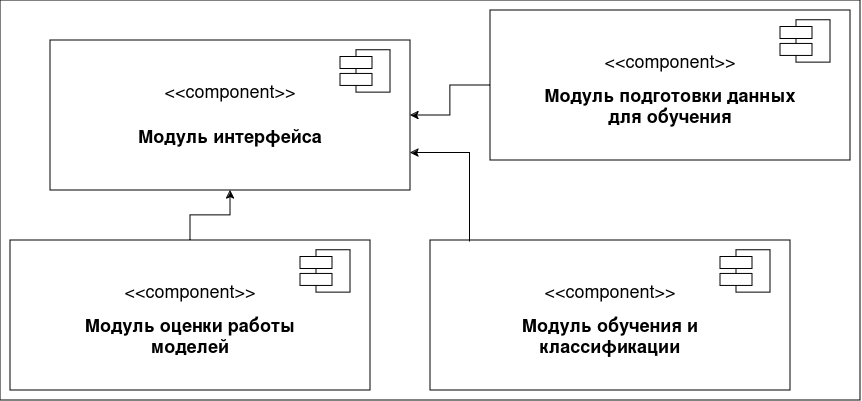
\includegraphics[width=1\linewidth]{pic/architecture.png}
    \vspace{-1em}\caption{Архитектура приложения}
    \label{ris:architecture}
\end{figure}
\vspace{1em}

\textit{Головной модуль} представляет собой главный модуль для отображения работы с работой веб-интерфейсом, с которым пользователь может взаимодействовать, и осуществляет работу модулей по работе с моделями.

\textit{Модуль подготовки данных для обучения} отвечает за подготовку и предобработку данных, необходимых для обучения моделей машинного обучения. Включает в себя различные этапы предварительной обработки данных, такие как удаление выбросов, выбор и сортирование критериев репозиториев.

\textit{Модуль классификации} отвечает за определение класса популярности проекта. Он принимает на вход предварительно подготовленные данные и выбранную модель классификации, а затем определяет класс популярности проекта по модели. Модуль классификации также может работать с модулем оценки работы за счет выбранной модели.

\textit{Модуль регрессии} отвечает за прогнозирование количества звезд относительно других параметров проекта с использованием различных моделей машинного обучения. Он принимает на вход предварительно подготовленные данные и выбранную модель регрессии, а затем выполняет прогнозирование целевых числовых значений. Модуль регрессии также может работать с модулем оценки работы за счет выбранной модели, т.е. проводить оценку качества регрессии.

\textit{Модуль оценки работы моделей} отвечает за оценку эффективности работы различных моделей машинного обучения. Включает в себя запуск алгоритмов оценки с использованием предварительно загруженных данных, разделенных на обучающий и тестовый наборы. Модуль оценки работы моделей запускает процессы обучения и тестирования моделей классификации и регрессии, сравнивая их результаты с заданными метриками, такими как точность, полнота, F1-мера, MSE и другими. 

\subsection{Проектирование пользовательского интерфейса}
\label{sec:Graphical-interface}

В данном разделе будут представлены спроектированные макеты пользовательского интерфейса приложения. Данные макеты являются примерным представлением итогового продукта и содержат в себе основные необходимые функции.

Для разрабатываемого приложения было решено создать простой и интуитивно понятный интерфейс для удобства пользователя.

Главная страница содержит в себе форму выбора типа модели: модели классификации, которая отвечает за определение класса популярности проекта по заданным параметрам, и модели регрессии, которая прогнозирует возможный результат значения параметра "звезды". Также на форме будет кнопка для перехода на страницу с вводом параметров и выбранным типом модели. Макет формы на главной странице представлен на рисунке~\ref{ris:main-form}.

\begin{figure}[h]
    \centering
    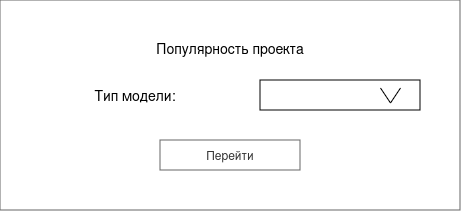
\includegraphics[width=0.7\linewidth]{pic/main-form.png}
    \vspace{0.5em}\caption{Макет формы выбора типа модели}
    \label{ris:main-form}
\end{figure}
\vspace{1em}

Страница для моделей классификации и моделей регрессии выглядит одинаково, содержит в себе форму для отправки данных. Окно содержит поля для данных по параметрам проекта, включая имя репозитория и численных характеристики. А также выбор модели из выпадающего списка для определения класса популярности и кнопку, которая переадресует на другую страницу с результатами. На странице модели классификации также содержится поле для ввода звезд. На рисунке~\ref{ris:form-input} представлен макет формы ввода.

\begin{figure}[h]
    \centering
    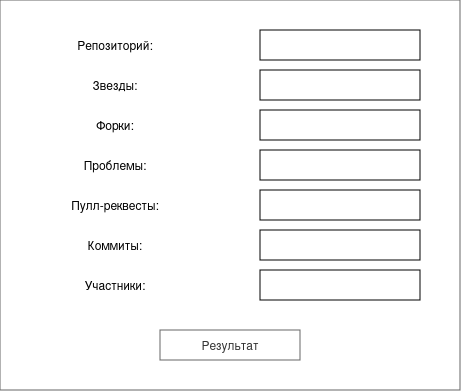
\includegraphics[width=0.8\linewidth]{pic/form-input.png}
    \vspace{0.5em}    \caption{Макет формы ввода параметров проекта}
    \label{ris:form-input}
\end{figure}
\vspace{1em}

Страница c результатом определения класса популярности проекта содержит в себе форму с определенным классом в виде числа от 0 до 10. Так на странице ввыведена та же информация, что была представлена для классификации, в качестве указания на то, что система верно интерпретировала данные. На рисунке~\ref{ris:result-form} представлен макет результата определения класса. Страница с определением количеством звезд проекта представлена аналогично.

\begin{figure}[h]
    \centering
    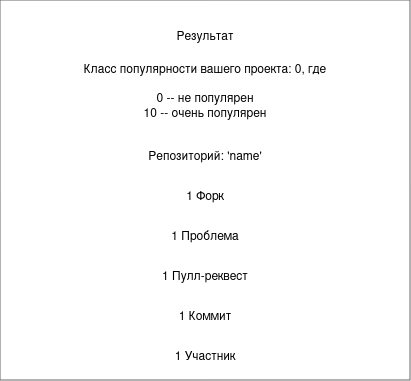
\includegraphics[width=0.8\linewidth]{pic/result-form.png}
    \vspace{0.5em}    \caption{Макет формы результата класса популярности}
    \label{ris:result-form}
\end{figure}
\vspace{1em}
